\chapter{Implementazione}

\textit{In questo capitolo viene descritto il lavoro di implementazione svolto, mostrando come le scelte progettuali illustrate nel capitolo precedente
si sono tradotte in codice effettivo.}
\section{Sistema di persistenza a superfile} \label{sec:impl-superfile}

\subsection{Richiamo alla scelta progettuale}

Questa sezione traduce in codice l'architettura del superfile descritta in
\hyperref[sec:superfile]{Sistema di persistenza a superfile}: la separazione tra
formato su disco e stato di runtime, le operazioni di creazione, apertura con
recovery, scrittura, sincronizzazione e chiusura, la finestra di azzeramento
anticipata a supporto della recovery e la comunicazione dello stato di occupazione.

\subsection{Strutture dati e interfacce}

Il formato su disco descritto in progettazione elencava nove campi logici
dell'header. Nella struttura effettivamente persistita, tuttavia, ne compaiono
solo alcuni:

\begin{listing}[H]
\begin{minted}{cpp}
struct Header {
    uint32_t magic;             // costante di validita' ("EGL1")
    uint8_t  version;
    uint32_t dataStartOffset;
    uint32_t dataEndOffset;
    uint32_t recordCount;
    uint8_t  wrapped;
};
\end{minted}
\caption{Header effettivamente persistito su disco}
\label{listing:header-disco}
\end{listing}

La scelta è giustificata: solo i campi che \emph{variano nel tempo} e non sono
altrimenti ricostruibili vengono scritti su microSD; tutto ciò che è invece
 derivabile dal firmware in esecuzione viene ricalcolato a
ogni apertura, evitando di duplicare un'informazione che potrebbe disallinearsi
dalla sua sorgente (le costanti del firmware). La Tabella
\ref{tab:header-logico-persistito} riassume la corrispondenza.

\begin{table}[H]
\centering
\begin{tabular}{l c l}
\hline
\textbf{Campo logico} & \textbf{Persistito} & \textbf{Se non persistito, ricavato da} \\
\hline
Versione del formato & Sì & --- \\
Identificativo del sensore & No & nome del file (\texttt{buildPath}) \\
Dimensione del record & No & \texttt{getSensorParams(sensorId)} \\
Capacità totale & No & \texttt{computeTotalRecords(...)} \\
Cursore di fine dati & Sì & --- \\
Cursore di inizio dati & Sì & --- \\
Soglia di sincronizzazione & No & \texttt{HEADER\_SYNC\_BYTES\_TARGET/recordSize} \\
Dim. finestra di azzeramento & No & \texttt{syncEveryRecords * 2} \\
Indicatori di stato & Parziale & \texttt{wrapped} persistito; \texttt{isFull} ricalcolato \\
\hline
\end{tabular}
\caption{Corrispondenza tra i campi logici dell'header e la loro effettiva persistenza}
\label{tab:header-logico-persistito}
\end{table}

Il motivo comune alla maggior parte dei campi non persistiti è il costo delle
operazioni di scrittura: l'header non viene risincronizzato a ogni record, ma
periodicamente (\hyperref[subsec:sincronizzazione_header]{Sincronizzazione
dell'header}), quindi ogni campo incluso nell'area persistita viene riscritto
a ogni sincronizzazione per l'intera durata della sessione. Un valore che non
cambia mai, o che cambia solo alla creazione del file, comporterebbe un costo
ricorrente per un'informazione di fatto statica. Nel dettaglio:

\begin{itemize}
    \item \textbf{Identificativo del sensore}: già codificato nel nome del
    file; ripeterlo nell'header sarebbe ridondante.
    \item \textbf{Dimensione del record}: dipende esclusivamente dal tipo di
    sensore ed è fissata a livello di firmware, come anche l'\gls{odr} dei 
    sensori, la finestra di retention e i pin logici usati dai vari moduli.
    \item \textbf{Capacità totale}: dipende da parametri di configurazione firmware,
     invarianti per l'intera vita del file; ricalcolarla
    costa poche operazioni aritmetiche, contro un campo che andrebbe scritto
    una sola volta e mai più aggiornato.
    \item \textbf{Soglia di sincronizzazione}: deriva dalla dimensione del
    record e da una costante di firmware; persisterla vincolerebbe il file al
    valore scelto alla creazione anche a fronte di un futuro aggiornamento
    firmware.
    \item \textbf{Dimensione della finestra di azzeramento}: deriva
    interamente dalla soglia di sincronizzazione, stessa motivazione del punto
    precedente.
    \item \textbf{Indicatori di stato}: rispetto ai due esempi previsti in 
    progettazione per questo campo logico, ovvero l’abilitazione dell’overwrite 
    e il raggiungimento della capacità massima, l’abilitazione dell’overwrite è 
    in realtà una costante per sensore (Tabella \ref{tab:constants-per-sensore})
     anziché un campo dell’header. \texttt{wrapped} costituisce invece un ulteriore 
     indicatore, non anticipato in progettazione ma della stessa natura concettuale, 
     ed è persistito perché rappresenta un evento realmente accaduto sul supporto
      (un giro completo del buffer) che nessun ricalcolo potrebbe altrimenti ricostruire. 
      \texttt{isFull} è invece sempre deducibile confrontando \texttt{recordCount} 
      con la capacità totale, quindi persisterlo aggiungerebbe un’informazione 
      ridondante da mantenere sincronizzata a ogni scrittura.
\end{itemize}

Questa equivalenza tra ricalcolo e rilettura regge perché la recovery avviene
sempre nello stesso firmware con cui il file era stato creato: un riavvio non
cambia le costanti di configurazione.

Due campi compaiono nella struttura persistita senza comparire tra i nove
campi logici elencati in progettazione. 

Il primo è la \textbf{costante magica} (\texttt{magic}), scritta all'inizio 
dell'header e verificata a ogni apertura insieme alla versione: a differenza 
degli altri campi non descrive lo stato del file, ma ne attesta la validità 
prima di fidarsi del resto del contenuto, distinguendo un header corretto da 
uno corrotto o mai inizializzato. 

Il secondo è \texttt{recordCount}: ridondante rispetto ai due soli cursori, ma
necessario per distinguere senza ambiguità un buffer vuoto da uno pieno, casi
in cui \texttt{dataStartOffset} e \texttt{dataEndOffset} coinciderebbero
altrimenti. \\

Lo stato di runtime (\texttt{Instance}) mantiene invece il riferimento al file
aperto, i parametri ricalcolati sopra elencati e i contatori di servizio
(\texttt{recordsSinceSync}). Le operazioni concettuali di progettazione sono
realizzate come funzioni libere che operano su un'istanza esplicita, senza
stato nascosto:

\begin{listing}[H]
\begin{minted}{cpp}
bool create(SdFat& sdFat, Instance& inst, const char* path,
            uint32_t recordSize, uint32_t totalRecords,
            uint32_t headerAreaSize, bool allowOverwrite);

bool openAndRecover(SdFat& sdFat, Instance& inst, const char* path, /* ... */);

bool writeRecords(Instance& inst, const uint8_t* src, uint32_t count);
bool syncHeader(Instance& inst);
void close(Instance& inst);
\end{minted}
\caption{Interfaccia del modulo superfile (\texttt{openAndRecover} condivide gli stessi parametri di \texttt{create}, omessi per brevità)}
\label{listing:superfile-interface}
\end{listing}

\subsection{Dettagli implementativi}

\paragraph{Creazione e calcolo della capacità}
La capacità totale, descritta in
\hyperref[subsec:capacita_superfile]{Capacità del file}, è calcolata
arrotondando per eccesso alla dimensione del cluster del volume. In questo
modo, la dimensione del superfile viene allineata, per quanto possibile, alla
granularità di allocazione della scheda microSD, evitando di lasciare
porzioni di spazio inutilizzate all’interno dell’ultimo cluster allocato e
riducendo al minimo la frammentazione del file system. L’obiettivo è quindi
fare in modo che le operazioni di allocazione e gestione dello spazio siano
quanto più possibile allineate ai cluster fisici della scheda:

\begin{listing}[H]
\begin{minted}{cpp}
uint64_t rawBytes = uint64_t(hz) * 3600ULL * retentionHours * recordSize;
uint64_t alignedBytes = ((rawBytes + clusterSizeBytes - 1) / clusterSizeBytes)
* clusterSizeBytes;
return uint32_t(alignedBytes / recordSize);
\end{minted}
\caption{Calcolo della capacità del superfile}
\label{listing:compute-total-records}
\end{listing}

I parametri da cui questi valori
derivano (\texttt{hz}, \texttt{retentionHours}, dimensione del
record e pin logici) sono centralizzati in un unico
file di configurazione firmware, \texttt{constants.h}, anziché essere sparsi
tra i singoli moduli sensore: una modifica alla frequenza di campionamento o
alla finestra di retention di un sensore richiede quindi di intervenire in
un solo punto del codice. La Tabella \ref{tab:constants-per-sensore} riporta i
valori concreti attualmente configurati per ciascun sensore.

\begin{table}[H]
\centering
\begin{tabular}{l c c c c}
\hline
\textbf{Sensore} &
\textbf{ODR} &
\textbf{\makecell{RETENTION\\HOURS}} &
\textbf{\makecell{ALLOW\\OVERWRITE}} &
\textbf{\makecell{FLUSH\\INTERVAL\_S}} \\
\hline
Barometro    & 1 Hz   & 10 h & sì & 120 s\\
Magnetometro & 1 Hz   & 10 h & sì & 5 s  \\
IMU          & 417 Hz & 10 h & sì & 8 s  \\
GPS          & 10 Hz  & 20 h & no & 48 s \\
\hline
\end{tabular}
\caption{Parametri concreti per sensore definiti in \texttt{constants.h}}
\label{tab:constants-per-sensore}
\end{table}

\paragraph{Scrittura e wraparound}
Quando il blocco da scrivere attraversa il limite superiore dell'area dati,
la scrittura viene spezzata in due parti, come descritto in progettazione:

\begin{listing}[H]
\begin{minted}{cpp}
// wraparound: split in scrittura pre-wrap e post-wrap
uint32_t firstPartRecords = recordsToWrapBoundary;
uint32_t secondPartRecords = writable - firstPartRecords;

file.write(src, firstPartRecords * recordSize);     // fino a fine area dati
file.write(src + firstPartRecords * recordSize,
           secondPartRecords * recordSize);         // dall'inizio dell'area dati
\end{minted}
\caption{Split della scrittura in caso di wraparound (gestione errori omessa per brevità)}
\label{listing:wraparound}
\end{listing}

Per il sensore GPS, in modalità non-overwrite, al raggiungimento della
capacità massima le scritture successive vengono silenziosamente ignorate e
l'header viene marcato pieno, propedeuticamente alla terminazione automatica
della sessione già descritta in progettazione.

\paragraph{Sincronizzazione e finestra di azzeramento}
Ogni sincronizzazione dell'header ricostituisce la finestra di azzeramento a
partire dal nuovo cursore. La dimensione della finestra è pari al doppio della
soglia di sincronizzazione: poiché la finestra viene consumata progressivamente
tra una sincronizzazione e la successiva, raddoppiarla garantisce che, anche
immediatamente prima di un \textit{sync}, resti sempre almeno un intero intervallo di
sincronizzazione di record pre-azzerati davanti al cursore.

\paragraph{Recovery su più livelli}
La recovery descritta in \hyperref[subsec:Recovery]{Recovery dopo interruzioni
impreviste} è realizzata su tre livelli distinti: a livello di dispositivo
(\texttt{SD::recover()}) rimonta il file system, ricarica la configurazione e,
se una sessione risulta attiva, delega a un secondo livello
(\texttt{recoverAllForSession}) che itera tutti i sensori della sessione sotto
un unico lock; per ciascuno di essi invoca infine \texttt{openAndRecover},
che a livello di singolo file esegue la riconciliazione:

\begin{listing}[H]
\begin{minted}{cpp}
for (uint32_t i = 0; i < inst.zeroWindowRecords; i++) {
    uint64_t ts = 0;
    if (!readRecordTimestamp(inst, inst.header.dataEndOffset, ts)) break;
    if (ts == 0) break;              // primo record non ancora scritto: confine trovato
    advanceAfterAppend(inst);
}
\end{minted}
\caption{Riconciliazione del cursore in fase di recovery}
\label{listing:reconcile}
\end{listing}

\paragraph{Comunicazione dello stato di occupazione}
Come descritto in \hyperref[subsec:storage_status]{Comunicazione dello stato di
occupazione}, il calcolo è isolato in un componente separato dal modulo di persistenza,
invocato dal consumer subito dopo ogni scrittura riuscita e a ogni controllo di
presenza della scheda. Il valore condiviso con l'app raggruppa, per ciascun sensore, la
percentuale di occupazione e un indicatore di sovrascrittura in corso, oltre a un
indicatore complessivo di assenza della scheda; viene reso disponibile al sottosistema BLE
come singolo valore sempre sovrascritto, coerentemente con la scelta di trattarlo come
\textit{snapshot} più recente piuttosto che come sequenza di eventi da accodare.

\subsection{Problematiche riscontrate e soluzioni}

Nella fase iniziale del tirocinio erano disponibili due prototipi: uno con i
componenti saldati e uno su breadboard. Su quest'ultimo, il contatto poco
affidabile del pin \texttt{DET} dello slot microSD produceva un errore
particolarmente insidioso: la scheda veniva segnalata come inserita anche
quando fisicamente assente.

\begin{listing}[H]
\begin{minted}{cpp}
// Prima: stato meccanico del pin DET
bool isCardInserted() {
    return digitalRead(SD::PIN_DET);
}
\end{minted}
\caption{Rilevamento della scheda basato sul pin DET}
\label{listing:det-before}
\end{listing}

\begin{listing}[H]
\begin{minted}{cpp}
// Dopo: prova elettrica reale della scheda via SPI
bool isCardInserted() {
    auto* card = sdFat.card();
    if (!card) return false;
    cid_t cid;
    return card->readCID(&cid);
}
\end{minted}
\caption{Rilevamento della scheda tramite lettura del CID}
\label{listing:det-after}
\end{listing}

Questo tipo di falso positivo è più pericoloso del suo opposto: un falso
negativo si traduce semplicemente in un'attesa e in un nuovo tentativo, mentre
un falso positivo lascia proseguire il firmware oltre il controllo pensato
per impedire l'accesso in assenza di scheda, facendo fallire in modo meno
prevedibile le operazioni di apertura o scrittura successive. La lettura del
\gls{CID}, richiedendo una transazione \gls{SPI} che riesce solo se una scheda è
fisicamente presente e risponde correttamente, sposta il controllo dallo stato
meccanico di un contatto alla prova elettrica reale della sua operatività,
risultando affidabile su entrambi i prototipi indipendentemente dalla qualità
del contatto fisico. Il costo aggiuntivo, ossia l'esecuzione sotto lock SPI
anziché una lettura diretta di pin, è coerente con l'intervallo di polling già
in uso nel consumer.

\newpage

\section{Stato globale del dispositivo}

\subsection{Richiamo alla scelta progettuale}

Questa sezione traduce in codice quanto descritto in
\hyperref[sec:stato-globale]{Stato globale del dispositivo}: un punto di
accesso unico allo stato del dispositivo, in cui nessun componente mantiene
una propria copia locale delle informazioni condivise (\emph{Single Source of
Truth}), e in cui ogni indicatore è protetto da accessi concorrenti senza
bisogno di un lock esplicito.

\subsection{Strutture dati e interfacce}

Lo stato principale della sessione è rappresentato da un unico valore enumerato,
che può assumere uno dei cinque stati mutuamente esclusivi definiti in fase di
progettazione:

\begin{listing}[H]
\begin{minted}{cpp}
enum class State : uint8_t {
STAND_BY, LOGGING, SUSPENDED, DOWNLOADING, DELETING
};

State getCurrentState();
void setCurrentState(State s);
\end{minted}
\caption{Stato principale di sessione}
\label{listing:session-state}
\end{listing}

Gli altri indicatori (SD mancante, errore, calibrazione in corso, pairing,
download e cancellazione) sono invece rappresentati da booleani indipendenti,
ciascuno con una propria coppia di funzioni per la lettura e la modifica:

\begin{listing}[H]
\begin{minted}{cpp}
bool isSdMissing();
void setSdMissing(bool value);
\end{minted}
\caption{Interfaccia di un indicatore booleano indipendente}
\label{listing:global-state-indicator}
\end{listing}

Ogni altro indicatore segue lo stesso schema, omesso per brevità.\\

La scelta di un unico valore enumerato, anziché di un booleano indipendente per
ciascuno dei cinque stati, deriva dalla loro natura mutuamente esclusiva: il
dispositivo non può trovarsi contemporaneamente, ad esempio, in
\texttt{LOGGING} e \texttt{DOWNLOADING}. Un valore enumerato garantisce tale
vincolo direttamente a livello di rappresentazione, poiché l’impostazione di
un nuovo stato sostituisce quello precedente.

Gli indicatori booleani sono invece appropriati per condizioni ortogonali allo
stato principale: una condizione di errore o l’assenza della scheda microSD,
ad esempio, possono verificarsi indipendentemente dallo stato corrente.

\subsection{Dettagli implementativi}

\paragraph{Accesso senza lock}
Ogni variabile di stato è dichiarata come \texttt{std::atomic}, cioè come un
tipo che la libreria standard c++ garantisce come leggibile e scrivibile da più task
contemporaneamente:

\begin{listing}[H]
\begin{minted}{cpp}
std::atomic<bool> sdMissing{false};

bool isSdMissing() { return sdMissing.load(); }
void setSdMissing(bool v) { sdMissing.store(v); }
\end{minted}
\caption{Un indicatore come variabile atomica}
\label{listing:atomic-indicator}
\end{listing}

Questo evita di dover proteggere ogni lettura o scrittura con un mutex, come
sarebbe invece necessario se lo stato fosse raggruppato in un'unica struttura
non atomica: ogni indicatore è una variabile a sé, indipendente dalle altre,
quindi due componenti possono leggere o scrivere indicatori diversi nello
stesso istante senza mai doversi attendere a vicenda.

\paragraph{Un caso concreto: due task sullo stesso indicatore}
L'indicatore \texttt{sdMissing} viene scritto dal task consumer ogni volta che 
rileva un cambiamento nella presenza della scheda, e viene letto dal task che 
gestisce il LED, per decidere se mostrare
la segnalazione di massima priorità prevista dalla
Tabella \ref{tab:led-priorita}. Si tratta di due task completamente
indipendenti, che non comunicano tra loro in alcun altro modo:

\begin{listing}[H]
\begin{minted}{cpp}
// Task che gestisce la scrittura su SD
if (!cardInserted) {
    GlobalState::setSdMissing(true);
}
\end{minted}
\caption{Scrittura dell'indicatore da parte del task consumer}
\label{listing:sdmissing-writer}
\end{listing}

\begin{listing}[H]
\begin{minted}{cpp}
// Task che gestisce il LED, eseguito periodicamente
if (GlobalState::isSdMissing()) {
    return {255, 0, 0, PatternType::BLINK, 4.0f};
}
\end{minted}
\caption{Lettura dello stesso indicatore da parte del task LED}
\label{listing:sdmissing-reader}
\end{listing}

Il task LED non riceve alcuna notifica dal task consumer, né mantiene una propria
copia di "SD mancante": si limita a interrogare, ogni volta che deve decidere
cosa mostrare, la stessa variabile che il task consumer aggiorna.

\newpage

\section{Segnalazione di stato tramite LED}

\subsection{Richiamo alla scelta progettuale}

Questa sezione traduce in codice l'architettura a tre livelli descritta in
\hyperref[sec:led]{Segnalazione di stato tramite LED}: livello hardware,
livello decisionale e livello di rendering.

\subsection{Strutture dati e interfacce}

Il pattern visivo è rappresentato come dato immutabile, indipendente sia dalla
logica di decisione sia dal rendering:

\begin{listing}[H]
\begin{minted}{cpp}
enum class PatternType : uint8_t { SOLID, BLINK, BREATHING };

struct Pattern {
    uint8_t r, g, b;
    PatternType type;
    float frequencyHz; // usato solo per BLINK/BREATHING
};
\end{minted}
\caption{Value Object del pattern visivo}
\label{listing:led-pattern}
\end{listing}

I tre livelli sono realizzati come tre punti di ingresso distinti e non
interdipendenti: \mintinline{cpp}{LED::showColor(r, g, b)} sul livello
hardware, \mintinline{cpp}{LED::resolvePattern()} sul livello decisionale, e
un task periodico che richiama entrambi sul livello di rendering.

\subsection{Dettagli implementativi}

\paragraph{Livello decisionale}
La funzione \texttt{resolvePattern} implementa l'ordine di priorità della
Tabella \ref{tab:led-priorita} come una sequenza di controlli a cascata, in
cui il primo che risulta vero determina il pattern restituito:

\begin{listing}[H]
\begin{minted}{cpp}
Pattern resolvePattern() {
    if (GlobalState::isSdMissing())
        return {255, 0, 0, PatternType::BLINK, 4.0f};      // 1: SD mancante
    if (GlobalState::isError())
        return {255, 0, 0, PatternType::BLINK, 1.0f};      // 2: errore
    if (GlobalState::isPairingBle())
        return {0, 0, 255, PatternType::BLINK, 1.0f};      // 3: pairing BLE
    if (GlobalState::isPairingWifi())
        return {0, 0, 255, PatternType::BLINK, 4.0f};      // 4: pairing Wi-Fi
    if (GlobalState::isRetrievingData())
        return {255, 255, 0, PatternType::SOLID, 1.0f};    // 5: recupero dati
    if (GlobalState::isCalibrating())
        return {255, 255, 0, PatternType::BREATHING, 1.0f};// 6: calibrazione
    // ... download/cancellazione, sospensione, logging, standby
}
\end{minted}
\caption{Risoluzione del pattern per priorità esplicita (troncato per brevità)}
\label{listing:resolve-pattern}
\end{listing}

La struttura a cascata rende la Tabella \ref{tab:led-priorita} direttamente
leggibile nel codice: l'ordine dei controlli è l'ordine di priorità,
senza bisogno di una struttura dati o di un meccanismo di confronto separato.

\paragraph{Livello di rendering}
Il task di rendering richiama \texttt{resolvePattern()} periodicamente e
traduce il risultato in un'animazione effettiva. Un cambio di pattern fa ripartire 
da zero la fase dell'animazione, cosicché ogni
transizione di stato, ad esempio l'inizio di un lampeggio, parta sempre dal
proprio fronte iniziale invece che da un punto arbitrario del ciclo
precedente:

\begin{listing}[H]
\begin{minted}{cpp}
if (changed) {
    lastPattern = p;
    phaseStartMs = millis();
}
uint32_t elapsed = millis() - phaseStartMs;
\end{minted}
\caption{Aggancio della fase dell'animazione al cambio di pattern}
\label{listing:led-phase}
\end{listing}

Per \texttt{BLINK} la fase determina semplicemente se il tempo trascorso
ricade nella prima o nella seconda metà del periodo; per \texttt{BREATHING}
la stessa fase viene invece usata come argomento di una funzione sinusoidale,
che modula la luminosità del colore in modo continuo anziché a scatti.

\paragraph{Livello hardware}
Il livello hardware si riduce all'interfacciamento con la libreria del
LED sulla scheda, con due sole funzioni esposte al resto del firmware:

\begin{listing}[H]
\begin{minted}{cpp}
bool setupModule();                          // inizializza il LED
void showColor(uint8_t r, uint8_t g, uint8_t b);  // imposta un colore RGB
\end{minted}
\caption{Interfaccia del livello hardware}
\label{listing:led-hardware}
\end{listing}

Nessun dettaglio della libreria sottostante trapela oltre questa interfaccia: il
livello decisionale e quello di rendering, descritti di seguito, non sanno né
devono sapere quale libreria o quale LED fisico sia effettivamente in uso.

\newpage

\section{Gestione dell'inattività dei sensori}

\subsection{Richiamo alla scelta progettuale}

Questa sezione traduce in codice quanto descritto in
\hyperref[sec:inattivita]{Gestione dell'inattività dei sensori}: la sorgente
autorevole commutabile tra GPS e IMU, il debounce basato su campioni
consecutivi, e l'esclusione del GPS dalla sospensione.

\subsection{Strutture dati e interfacce}

Il modulo espone poche funzioni, ciascuna invocata da un punto preciso del
firmware: il producer GPS riporta ogni campione ricevuto, il producer IMU
riporta l'esito del proprio controllo di fallback, mentre il resto del
firmware può solo interrogare quale sorgente sia autorevole in un dato
istante:

\begin{listing}[H]
\begin{minted}{cpp}
void reportGpsSample(bool hasFix, float speedMps);
void reportImuFallbackSample(bool motionDetected);
bool isGpsAuthoritative();
uint32_t getTimeoutMs();
\end{minted}
\caption{Interfaccia del modulo di gestione dell'inattività}
\label{listing:inactivity-interface}
\end{listing}

\subsection{Dettagli implementativi}

\paragraph{Sorgente autorevole}
La funzione di decisione si riduce al confronto tra l'istante dell'ultimo fix
GPS e una soglia di freschezza: se il fix è recente, il GPS governa la
decisione di sospensione; altrimenti il compito passa all'IMU.

\begin{listing}[H]
\begin{minted}{cpp}
bool isGpsAuthoritative() {
    uint32_t lastFix = lastGpsFixMillis.load();
    if (lastFix == 0) return false;
    return (millis() - lastFix) <= GPS_FIX_FRESHNESS_MS;
}
\end{minted}
\caption{Determinazione della sorgente autorevole}
\label{listing:gps-authoritative}
\end{listing}

Questa singola funzione è il punto centrale a cui ogni altra parte del
sistema si appoggia per sapere quale sorgente considerare valida in un dato
momento, coerentemente con la scelta progettuale di centralizzare la
selezione pur mantenendo i due percorsi di rilevamento indipendenti.

\paragraph{Debounce sul segnale GPS}
Il rilevamento del movimento da GPS richiede un numero minimo di campioni
consecutivi sopra soglia prima di essere accettato, azzerando il conteggio a
ogni campione sotto soglia:

\begin{listing}[H]
\begin{minted}{cpp}
if (speedMps >= GPS_SPEED_THRESHOLD_MPS) {
    if (++consecutiveAboveThreshold >= GPS_MOTION_DEBOUNCE_SAMPLES) {
        resume();
    }
} else {
    consecutiveAboveThreshold = 0;
}
\end{minted}
\caption{Debounce del segnale di movimento GPS (semplificato)}
\label{listing:gps-debounce}
\end{listing}

\paragraph{Soglie e parametri di temporizzazione}
Il meccanismo si appoggia a quattro parametri, tutti tarati empiricamente: 
\begin{itemize}
    \item \texttt{GPS\_SPEED\_THRESHOLD\_MPS} (velocità GPS, $0.8\,\text{m/s}$, circa
        $2.9\,\text{km/h}$): sopra questo valore un campione GPS è considerato indicativo di movimento;
    \item \texttt{IMU\_ACCEL\_VARIANCE\_THRESHOLD} (varianza
        dell'accelerazione, circa 1.7g): soglia equivalente usata dal fallback IMU quando il GPS non è autorevole;
    \item \texttt{GPS\_FIX\_FRESHNESS\_MS} ($3000\,\text{ms}$): intervallo massimo dall'ultimo fix entro cui
    il GPS è considerato autorevole;
    \item \texttt{GPS\_MOTION\_DEBOUNCE\_SAMPLES} (3): numero di campioni consecutivi sopra soglia 
    richiesti per confermare il movimento.
\end{itemize}

È stata fatta una prima taratura da banco, seguita da un affinamento sul campo, in condizioni di utilizzo 
reali sul motoveicolo. \\

\paragraph{Attivazione mirata del fallback IMU}
Il percorso di rilevamento basato su IMU non viene campionato in
continuazione, ma solo mentre il dispositivo è già sospeso e il GPS non
risulta autorevole: è il producer IMU stesso, nel proprio ciclo di attesa, a
decidere quando interrogare l'accelerometro:

\begin{listing}[H]
\begin{minted}{cpp}
bool isImuFallbackPoll = (state == SUSPENDED && !Inactivity::isGpsAuthoritative());
if (isImuFallbackPoll) {
    IMU::sampleFallbackMotion(); // calcola la varianza e chiama reportImuFallbackSample
}
\end{minted}
\caption{Campionamento mirato del fallback IMU nel producer}
\label{listing:imu-fallback-poll}
\end{listing}

Questo evita di consumare cicli sull'accelerometro nei momenti in cui la
sorgente autorevole è comunque il GPS o il dispositivo è già attivo, senza
per questo modificare la logica di selezione della sorgente, che resta
interamente delegata a \texttt{isGpsAuthoritative()}.

\paragraph{Sospensione esclude il GPS}
Sia \texttt{suspend()} sia \texttt{resume()} notificano solo i producer
diversi dal GPS:

\begin{listing}[H]
\begin{minted}{cpp}
void notifyNonGpsProducers(uint32_t bit) {
    for (auto& ctx : Sensor::getProducerContexts()) {
        if (ctx.spec->sensorId == Sensor::SensorId::GPS) continue;
        xTaskNotify(handles[i], bit, eSetBits);
    }
}
\end{minted}
\caption{Propagazione della sospensione a tutti i producer tranne il GPS}
\label{listing:notify-non-gps}
\end{listing}

Il producer GPS, dal canto suo, esce immediatamente dalla propria funzione di
attesa senza mai fermarsi, restando l'unico sensore sempre acquisito
indipendentemente dallo stato di sospensione.

\paragraph{Sospensione disabilitata}
Quando il timeout è configurato a zero, ogni campione GPS aggiorna
immediatamente l'istante di ultimo movimento e forza il dispositivo a
LOGGING, disabilitando di fatto la sospensione:

\begin{listing}[H]
\begin{minted}{cpp}
if (timeoutMs == 0) {
    lastMotionMillis = now;
    resume();
    return;
}
\end{minted}
\caption{Disattivazione della sospensione tramite timeout a zero}
\label{listing:inactivity-never}
\end{listing}

\newpage


\section{Protocollo di avvio e arresto della sessione}

\subsection{Richiamo alla scelta progettuale}

Questa sezione traduce in codice quanto descritto in
\hyperref[sec:avvio-arresto]{Protocollo di avvio e arresto della sessione}: i
comandi START, STOP e RESUME come valori di un insieme chiuso, e le sequenze
di avvio e arresto orchestrate sopra i moduli di superfile, stato
globale e calibrazione dell'altitudine.

\subsection{Strutture dati e interfacce}

I comandi provenienti dall'app sono un enum a tre valori, instradati da un
unico punto di gestione:

\begin{listing}[H]
\begin{minted}{cpp}
enum class Command : uint8_t { START, STOP, RESUME };

void handleCommand(Command cmd);
\end{minted}
\caption{Interfaccia del modulo sessione}
\label{listing:session-command}
\end{listing}

\subsection{Dettagli implementativi}

\paragraph{Un prerequisito: producer in grado di dormire}
Come descritto in \hyperref[sec:situazione-partenza]{Situazione di partenza},
il firmware ricevuto all'inizio del tirocinio avviava l'acquisizione dati
automaticamente all'accensione, senza attendere alcun comando. Introdurre un
comando esplicito di avvio e arresto ha richiesto quindi, a monte del
protocollo vero e proprio, un intervento sui task producer stessi: ciascuno
di essi doveva poter restare inattivo finché nessuna sessione è in corso, e
riattivarsi solo alla ricezione del comando di avvio, anziché acquisire dati
in modo incondizionato dal boot del dispositivo. Ogni producer, a ogni ciclo,
verifica quindi lo stato di sessione prima di procedere:

\begin{listing}[H]
\begin{minted}{cpp}
while (GlobalState::getCurrentState() != GlobalState::State::LOGGING) {
    xTaskNotifyWait(0x0, ULONG_MAX, &notif, portMAX_DELAY); // dorme finche' non arriva un segnale
}
\end{minted}
\caption{Attesa del producer finché non è in corso una sessione (semplificato)}
\label{listing:producer-dormant}
\end{listing}

Senza questa modifica preliminare, il concetto stesso di "avvio" e "arresto"
di una sessione sarebbe stato privo di effetto: i producer avrebbero
continuato a produrre dati indipendentemente da qualunque comando ricevuto.
Il protocollo descritto nel resto di questa sezione si appoggia interamente
su questa capacità dei producer di restare in attesa.

\paragraph{Comandi come valori instradati centralmente}
\texttt{handleCommand} riceve il comando già decodificato dal canale BLE e lo
instrada con un semplice switch sul valore ricevuto, senza che la logica di
sessione debba conoscere nulla del trasporto con cui il comando è arrivato:
la stessa funzione potrebbe essere invocata da un trigger diverso da BLE
senza alcuna modifica.

\paragraph{Avvio sessione}
Alla ricezione di START, se il dispositivo non è occupato in download o
cancellazione e non è già in sessione, vengono eseguiti in sequenza: un
tentativo di recovery della scheda; la generazione del nome della cartella di
sessione, combinando identificativo del dispositivo, timestamp di inizio e il
suffisso \texttt{\_ACTIVE}; la creazione di tutti i superfile tramite il
registro descritto in \hyperref[sec:impl-superfile]{Sistema di persistenza a
superfile}; l'esecuzione sincrona della calibrazione dell'altitudine, il cui
esito viene comunque scritto nei metadati di sessione anche in caso di
fallimento; infine la transizione a LOGGING e la riattivazione forzata dei
producer:

\begin{listing}[H]
\begin{minted}{cpp}
snprintf(folderName, sizeof(folderName), "%s_%s%s",
         chipIdStr, sessionStartPrefix, "_ACTIVE"); //1
SD::SuperFile::createAllForSession(SD::sdFat, folderName); //2
auto cal = Session::AltitudeCalibration::run(SessionBle::ALTITUDE_CAL_TIMEOUT_MS); //3
GlobalState::setCurrentState(GlobalState::State::LOGGING); //4
Inactivity::forceWakeProducers(); //5
\end{minted}
\caption{Sequenza di avvio sessione (semplificata)}
\label{listing:session-start}
\end{listing}

Ogni fase è protetta da un accesso esclusivo al canale SPI condiviso con
timeout configurabile: il fallimento di una qualsiasi fase imposta lo stato
di errore e interrompe l'avvio, senza proseguire alle fasi successive.

\paragraph{Arresto sessione}
Alla ricezione di STOP (o della richiesta di arresto automatico per
esaurimento spazio GPS), la sequenza di chiusura
segue il seguente ordine: se il dispositivo era sospeso, i
producer vengono prima riattivati forzatamente; viene richiesto lo
svuotamento sincrono dei buffer verso il meccanismo di scrittura; il firmware 
attende che la coda di scrittura sia completamente
smaltita prima di chiudere i superfile, per non perdere record ancora in
transito; infine la cartella di sessione viene rinominata sostituendo il
suffisso \texttt{\_ACTIVE} con un riferimento temporale di fine sessione, e lo
stato torna a STAND\_BY.

\begin{listing}[H]
\begin{minted}{cpp}
Sensor::requestForceFlushAndWait(FORCE_FLUSH_TIMEOUT_TICKS); //1
waitForQueueDrain(); //2
SD::SuperFile::closeAll(); //3
SD::sdFat.rename(oldFolder, newFolder); //4
GlobalState::setCurrentState(GlobalState::State::STAND_BY); //5
\end{minted}
\caption{Sequenza di arresto sessione (semplificata)}
\label{listing:session-stop}
\end{listing}

\paragraph{Notifica periodica dello stato di sessione}
Un timer software FreeRTOS (\texttt{statusTimer}), creato una sola volta all'inizializzazione 
del modulo, viene avviato alla transizione a LOGGING e fermato al ritorno a STAND\_BY. A ogni 
scadenza richiama \texttt{notifyStatus()}, che compone una struttura compatta (stato della sessione, 
secondi trascorsi dall'inizio sessione e numero di campioni) e la pubblica come notifica BLE dedicata.

\paragraph{Comando RESUME: risincronizzazione dopo la riconnessione BLE}
Una sessione prosegue sul dispositivo indipendentemente dallo stato della connessione 
BLE: se l'app si disconnette e si riconnette mentre una sessione è già in corso, non 
riceve alcuna informazione di stato fino al successivo scadere del timer periodico 
appena descritto. Alla ricezione di RESUME il firmware richiama direttamente 
\texttt{notifyStatus()}, ottenendo una risincronizzazione immediata senza attendere 
il ciclo del timer e senza alcuna transizione dell'enum di sessione, che resta sotto 
il controllo esclusivo di START e STOP.

\paragraph{Un caso particolare: l'arresto per spazio esaurito}
Come descritto in progettazione, l'arresto automatico per esaurimento dello
spazio GPS esegue la stessa sequenza di arresto appena descritta, con
un'unica differenza a monte: prima di avviarla, il firmware imposta un
indicatore dedicato, che permette all'app di distinguere, leggendo lo stato
di sessione, un arresto voluto dall'utente da uno automatico.

\newpage

\section{Calibrazione dell'altitudine}

\subsection{Richiamo alla scelta progettuale}

Questa sezione traduce in codice l'algoritmo di calibrazione descritto in
\hyperref[sec:calibrazione-altitudine]{Calibrazione dell'altitudine}:
raccolta campioni con filtro dei duplicati, calcolo di mediana e deviazione
standard, accettazione o scarto del gruppo, e timeout massimo complessivo.

\subsection{Strutture dati e interfacce}

Il risultato della calibrazione è un dato immutabile che distingue
esplicitamente un esito riuscito da un fallimento per timeout:

\begin{listing}[H]
\begin{minted}{cpp}
struct Result {
    bool  calibrated;
    float referencePressureHpa; // valido solo se calibrated == true
    bool  timedOut;
};

Result run(uint32_t timeoutMs);
\end{minted}
\caption{Interfaccia del modulo di calibrazione dell'altitudine}
\label{listing:altitude-cal-interface}
\end{listing}

Il valore di riferimento accettato viene poi reso disponibile globalmente in
lettura tramite \texttt{setReferencePressure}/\texttt{getReferencePressure},
protetto da una sezione critica anziché da un mutex, essendo consultato anche
dal producer del barometro a ogni campione.

\subsection{Dettagli implementativi}

\paragraph{Raccolta campioni e filtro duplicati}
L'algoritmo interroga ripetutamente l'ultimo campione disponibile dal
producer del barometro, scartando quelli il cui timestamp coincide con
l'ultimo già considerato:

\begin{listing}[H]
\begin{minted}{cpp}
Barometer::Sample s = Barometer::getLastSample();
bool goodSample = s.timestamp != 0 && s.timestamp != lastTimestamp;
\end{minted}
\caption{Filtro dei campioni duplicati tramite confronto del timestamp}
\label{listing:altitude-cal-dedupe}
\end{listing}

Questo evita che una lettura più lenta del ciclo di polling della
calibrazione porti a contare più volte lo stesso campione fisico, falsando
sia la mediana sia la deviazione standard.

\paragraph{Mediana, deviazione standard e accettazione del gruppo}
Raggiunto il numero di campioni richiesto, il gruppo viene ordinato per
estrarne la mediana, e la deviazione standard viene calcolata rispetto a
quest'ultima anziché rispetto alla media, coerentemente con la scelta della
mediana come stima robusta descritta in progettazione:

\begin{listing}[H]
\begin{minted}{cpp}
std::sort(sorted, sorted + N);
float median = sorted[N / 2];
for (auto v : samples) variance += (v - median) * (v - median);
float stddev = sqrtf(variance / N);

if (stddev <= MAX_STDDEV_HPA) {
    return Result{ true, median, false };
}
\end{minted}
\caption{Calcolo di mediana e deviazione standard, e criterio di accettazione}
\label{listing:altitude-cal-median}
\end{listing}

Se la deviazione standard supera la soglia prevista, l’intero insieme di campioni 
viene scartato e la raccolta viene riavviata da zero, in accordo con quanto definito 
in progettazione. Qualora, invece, il timeout complessivo scada senza che sia stato 
possibile ottenere un insieme di campioni valido, la funzione restituisce un risultato 
con \texttt{timedOut = true} e la sessione prosegue comunque, seppur priva di un 
riferimento di altitudine valido. Tale comportamento è coerente con i requisiti della 
calibrazione: essa è necessaria per ottenere un’altitudine relativa priva dell’errore 
sistematico dovuto alla quota iniziale, ma non costituisce una condizione vincolante 
per l’avvio o la prosecuzione della sessione.  

\paragraph{Formula di conversione e scelta del dato da conservare}

L'altitudine relativa a un dato istante è calcolata dalla formula
barometrica standard:

\begin{equation}
    h = 44330 \left( 1 - \left( \frac{p}{p_0} \right)^{\frac{1}{5.255}} \right)
    \label{eq:altitude-barometric}
\end{equation}

dove $h$ è l'altitudine relativa in metri, $p$ la pressione istantanea
misurata e $p_0$ la pressione di riferimento acquisita in fase di
calibrazione. La costante $44330$ rappresenta l'altezza approssimativa,
in metri, dell'atmosfera terrestre secondo il modello standard, mentre
l'esponente $1/5.255$ deriva dal tasso di variazione della pressione con
la quota previsto dallo stesso modello.\\

Il valore effettivamente conservato al termine della calibrazione, tuttavia,
non è un'altitudine già calcolata, ma la sola pressione di riferimento in
\gls{hpa}. La scelta è motivata dalla formula stessa: per restituire un'altitudine
priva di errore sistematico, il calcolo richiede sempre \emph{due} pressioni,
quella istantanea e quella di riferimento, non un singolo valore di quota
assoluta.

\newpage

\section{Calibrazione dell'IMU}

\subsection{Richiamo alla scelta progettuale}

Questa sezione traduce in codice quanto descritto in
\hyperref[sec:calibrazione-imu]{Calibrazione dell'IMU}: la macchina a stati
esplicita, il Command Pattern per i comandi dall'app, il fan-out non invasivo
sul flusso dati IMU, il retry isolato per singolo step, e l'algoritmo dei tre
step di misura.

\subsection{Strutture dati e interfacce}

Gli stati e i comandi sono rappresentati come due enum distinti, coerenti con
il Command Pattern e lo State Pattern descritti in progettazione:

\begin{listing}[H]
\begin{minted}{cpp}
enum class CalibCommand : uint8_t { START, CONFIRM, ABORT };

enum class CalibState : uint8_t {
    IDLE, 
    STEP1_READY, STEP1_RUNNING, STEP1_RETRY,
    STEP2_READY, STEP2_RUNNING, STEP2_RETRY,
    STEP3_READY, STEP3_RUNNING, STEP3_RETRY,
    SUCCESS, NO_DATA, ERR
};
\end{minted}
\caption{Comandi e stati della calibrazione IMU}
\label{listing:calib-states}
\end{listing}

Il campione grezzo duplicato dal producer verso il canale di calibrazione è
anch'esso una struttura minima, priva di qualunque elaborazione:

\begin{listing}[H]
\begin{minted}{cpp}
struct CalibSample {
    int32_t accel[3];
    int32_t gyro[3];
};
\end{minted}
\caption{Campione grezzo instradato al task di calibrazione}
\label{listing:calib-sample}
\end{listing}

\subsection{Dettagli implementativi}

\paragraph{Fan-out non invasivo sul flusso dati}
Il producer dell'IMU continua a funzionare come se la calibrazione non
esistesse: l'unica aggiunta è, quando la calibrazione è attiva, la
duplicazione di ogni campione verso una coda dedicata, senza alcuna modifica
al percorso di acquisizione ed elaborazione già in uso durante il logging:

\begin{listing}[H]
\begin{minted}{cpp}
if (IMU::isCalibrationActive()) {
    IMU::CalibSample calibSample;
    calibSample.accel[0] = currentSample.rawAccelX;
    // ... e le altre componenti
    xQueueSend(IMU::calibQueue(), &calibSample, 0);
}
\end{minted}
\caption{Duplicazione del campione verso il canale di calibrazione}
\label{listing:calib-fanout}
\end{listing}

\paragraph{Macchina a stati e instradamento dei comandi}
Un unico task consuma i comandi dalla coda e li interpreta in funzione dello
stato corrente, secondo un semplice switch a due livelli (stato, poi
comando), realizzando così sia lo State Pattern sia il Command Pattern
descritti in progettazione: l'esecuzione effettiva di uno step è sempre
delegata a una funzione comune, che riceve come parametri lo stato di
esecuzione, lo stato di retry, lo stato successivo e la funzione da eseguire,
disaccoppiando la sequenza delle transizioni dal contenuto di ciascuno step:

\begin{listing}[H]
\begin{minted}{cpp}
void runMeasuredStep(CalibState runningState, CalibState retryState,
                      CalibState nextReadyState,
                      CalibStepResult (*stepFn)(), bool isLastStep);
\end{minted}
\caption{Firma della funzione comune di esecuzione di uno step}
\label{listing:run-measured-step}
\end{listing}

Un solo indice (\texttt{activeStepIndex}) tiene traccia dello step
attualmente in corso: è ciò che permette, in caso di comando CONFIRM ricevuto
mentre lo stato è \texttt{NO\_DATA}, di sapere quale dei tre step ripetere,
poiché quello stato è raggiungibile da ciascuno dei tre step del percorso di
calibrazione.

\paragraph{Soglie di accettazione degli step}
Ciascuno dei controlli descritti nei paragrafi seguenti confronta una
grandezza misurata con una soglia fissa, riportata in
Tabella~\ref{tab:calib-thresholds}. I valori sono stati tarati empiricamente,
con una combinazione di prove da banco e prove sul campo, montando il dispositivo 
sul motoveicolo nelle condizioni reali di utilizzo. 

\begin{table}[H]
\centering
\small
\setlength{\tabcolsep}{5pt}
\renewcommand{\arraystretch}{1.2}
\begin{tabularx}{\textwidth}{>{\raggedright\arraybackslash}p{5.2cm}
                              >{\centering\arraybackslash}p{2.2cm}
                              X}
\hline
\textbf{Soglia} & \textbf{Valore} & \textbf{Utilizzo} \\
\hline
\texttt{STEP1\_GRAVITY\_MIN/MAX\_MG}
& 700--1300 mG
& Intervallo accettabile per il modulo di gravità misurato nello Step 1 \\
\texttt{STEP1\_STILL\_VARIANCE
\_THRESHOLD\_MG2}
& 17000 mG\textsuperscript{2}
& Varianza massima ammessa per considerare il dispositivo fermo nello Step 1 \\
\texttt{STEP2\_TILT\_MIN\_MG}
& 120 mG
& Componente laterale minima per considerare valida l'inclinazione dello Step 2 \\
\texttt{STEP3\_FWD\_MIN\_NORM}
& 0.1
& Modulo minimo dell'asse longitudinale calcolato, sotto cui la geometria è giudicata degenere \\
\texttt{EARLY\_EXIT\_STD\_DEV\_MG}
& 15 mG
& Soglia di stabilità del segnale per l'uscita anticipata da uno step \\
\hline
\end{tabularx}
\caption{Soglie di accettazione della calibrazione IMU}
\label{tab:calib-thresholds}
\end{table}

\paragraph{Uscita anticipata basata sulla stabilità del segnale}
Ogni step condivide la stessa routine di raccolta campioni, che integra un
periodo di assestamento iniziale (i campioni ricevuti in questa fase vengono
scartati) e un meccanismo di uscita anticipata: superato un numero minimo di
campioni, la deviazione standard del modulo dell'accelerazione viene
calcolata su una finestra scorrevole delle ultime letture, e se risulta sotto
soglia lo step termina subito, senza attendere il timeout completo:

\begin{listing}[H]
\begin{minted}{cpp}
if (count >= EARLY_EXIT_MIN_SAMPLES && windowCount == EARLY_EXIT_CHECK_WINDOW) {
    // media e deviazione standard sulla finestra di ultimi campioni
    if (windowStdDev < EARLY_EXIT_STD_DEV_MG) break; // segnale stabile: esce prima
}
\end{minted}
\caption{Uscita anticipata quando il segnale è già stabile (semplificato)}
\label{listing:calib-early-exit}
\end{listing}

\paragraph{Step 1 - Posizione dritta}
Con il dispositivo fermo, la media dei campioni raccolti approssima il vettore
di gravità così come misurato dal sensore. Il modulo di questo vettore deve
cadere in un intervallo plausibile attorno a 1 g, e la sua varianza deve
restare sotto una soglia di stabilità: al di fuori di questi limiti lo step
viene rifiutato, perché il dispositivo non era sufficientemente fermo o
orientato in modo anomalo. Se accettato, il vettore normalizzato diventa
l'asse verticale del sistema di riferimento, mentre lo scostamento del
vettore misurato rispetto a quello atteso (1 g lungo la verticale) diventa il
bias dell'accelerometro da sottrarre nelle acquisizioni successive; la media
dei campioni del giroscopio, che a dispositivo fermo dovrebbe essere nulla,
ne costituisce analogamente il bias.

\paragraph{Step 2 - Inclinazione a destra}
Il dispositivo viene inclinato lateralmente. Lo scostamento tra il vettore
medio misurato in questo step e quello registrato nello Step 1 viene
proiettato sul piano perpendicolare all'asse verticale già determinato,
isolando così la sola componente dello scostamento dovuta all'inclinazione
laterale, indipendentemente da eventuali piccole variazioni residue lungo la
verticale. Se il modulo di questa componente risulta troppo piccolo,
l'inclinazione è giudicata insufficiente e lo step viene rifiutato;
altrimenti, il vettore normalizzato diventa l'asse laterale.

\paragraph{Step 3 - Asse longitudinale e salvataggio}
Il terzo asse non richiede una nuova misura: è calcolato geometricamente come
prodotto vettoriale tra l'asse laterale e quello verticale già determinati,
il che garantisce per costruzione un sistema di riferimento ortogonale. Un
breve intervallo di raccolta campioni resta comunque necessario per
verificare che il flusso dati dal sensore sia ancora presente. Se il modulo
del vettore risultante è troppo piccolo, significa che i due assi precedenti
erano quasi paralleli tra loro, cioè che l'inclinazione dello Step 2 non era
sufficientemente distinta dalla posizione dello Step 1: una geometria
degenere, che comporta il rifiuto dello step. In caso di successo, i tre
assi compongono la matrice di rotazione salvata in configurazione insieme ai
bias calcolati nello Step 1.

\paragraph{Gestione degli esiti negativi}
I tre step condividono lo stesso schema di esito: nessun campione ricevuto
entro il timeout porta allo stato \texttt{NO\_DATA} (probabile problema
hardware, non di postura), un numero di campioni insufficiente o una
geometria/misura non valida porta allo stato di retry specifico dello step
corrente, mentre un comando di interruzione esplicita riporta immediatamente
lo stato a \texttt{IDLE} indipendentemente dallo step in corso.

\subsection{Problematiche riscontrate e soluzioni}

La soglia di varianza dello Step 1
(\texttt{STEP1\_STILL\_VARIANCE\_THRESHOLD\_MG2}) era stata inizialmente
tarata mediante prove da banco. Il primo test sul campo ha evidenziato che
tale taratura risultava ancora troppo restrittiva, poiché non teneva conto
delle vibrazioni trasmesse dal motoveicolo durante il funzionamento del
motore. La soglia è stata quindi ritarata sulla base delle condizioni reali
di utilizzo, considerando anche i tremolii rilevati con il mezzo fermo e il
motore acceso.

\newpage

\section{Architettura dello sniffer CAN}

\subsection{Richiamo alla scelta progettuale}

Questa sezione traduce in codice l'architettura esagonale descritta in
\hyperref[sec:sniffer-arch]{Architettura dello sniffer CAN}: le tre porte del
dominio, il caso d'uso che le orchestra senza conoscerne gli adattatori
concreti, e le implementazioni realizzate per il prototipo (bus CAN in
ascolto passivo, profilo Yamaha MT-07, trasporto via advertising BLE).

\subsection{Strutture dati e interfacce}

Le tre porte sono interfacce astratte pure, ciascuna con una responsabilità
unica:

\begin{listing}[H]
\begin{minted}{cpp}
class ICanBus {
public:
    virtual bool init() = 0;
    virtual bool receive(CanFrame& out, uint32_t timeoutMs) = 0;
};

class IVehicleProfile {
public:
    virtual uint8_t profileId() const = 0;
    virtual bool handleFrame(const CanFrame& frame) = 0;
    virtual TelemetrySnapshot currentSnapshot() const = 0;
};

class ITelemetryBroadcaster {
public:
    virtual bool init() = 0;
    virtual void publish(const TelemetrySnapshot& snapshot) = 0;
};
\end{minted}
\caption{Le tre porte del dominio}
\label{listing:sniffer-ports}
\end{listing}

Il dato scambiato tra bus e profilo (\texttt{CanFrame}) e quello scambiato
tra profilo e broadcaster (\texttt{TelemetrySnapshot}) sono entrambi
strutture dati semplici, prive di logica: il primo rispecchia un frame CAN
grezzo, il secondo lo stato di telemetria già decodificato e leggibile.

\subsection{Dettagli implementativi}
\paragraph{Il caso d'uso: orchestrazione senza conoscenza degli adattatori}
\texttt{SniffingService} riceve le tre porte nel costruttore come riferimenti
alle interfacce astratte, non alle classi concrete che le implementano:

\begin{listing}[H]
\begin{minted}{cpp}
class SniffingService {
public:
    SniffingService(ICanBus& bus, IVehicleProfile& profile,
                     ITelemetryBroadcaster& broadcaster)
        : bus_(bus), profile_(profile), broadcaster_(broadcaster) {}
private:
    ICanBus& bus_;
    IVehicleProfile& profile_;
    ITelemetryBroadcaster& broadcaster_;
};
\end{minted}
\caption{Costruzione del caso d'uso tramite le sole interfacce di dominio}
\label{listing:sniffer-service-ctor}
\end{listing}

In pratica, questa classe non sa mai quale bus CAN, quale profilo veicolo o
quale sistema di trasmissione stia realmente usando: conosce solo che
ciascuno di essi sa fare le operazioni previste dalla propria interfaccia
(ricevere un frame, interpretarlo, pubblicare un risultato). Decidere quali
classi concrete usare avviene altrove, nel punto in cui il firmware crea gli
oggetti: \texttt{SniffingService} non deve essere toccato nemmeno se si
cambia, ad esempio, il modo in cui i dati vengono trasmessi.

Il ciclo che sfrutta questa astrazione è invocato una volta per ogni
iterazione del \texttt{loop()} del firmware:

\begin{listing}[H]
\begin{minted}{cpp}
void loop() {
    sniffingService->tick(/*receiveTimeoutMs=*/10);
}
\end{minted}
\caption{Punto di chiamata del ciclo di orchestrazione}
\label{listing:sniffer-loop}
\end{listing}

Il corpo di \texttt{tick()} è breve:

\begin{listing}[H]
\begin{minted}{cpp}
void tick(uint32_t receiveTimeoutMs = 0) {
    CanFrame frame;
    if (!bus_.receive(frame, receiveTimeoutMs)) return;

    if (profile_.handleFrame(frame)) {
        broadcaster_.publish(profile_.currentSnapshot());
    }
}
\end{minted}
\caption{Ciclo di orchestrazione del caso d'uso}
\label{listing:sniffer-tick}
\end{listing}

Un frame CAN viene ricevuto, passato al profilo veicolo perché lo interpreti,
e solo se il profilo riconosce quell'identificativo (\texttt{handleFrame()}
restituisce vero) il risultato aggiornato viene pubblicato. I frame che non
appartengono a nessun segnale noto per quel veicolo vengono quindi ignorati,
senza generare alcuna pubblicazione.

\paragraph{Adattatore del bus CAN: ascolto passivo}
L'adattatore concreto della porta \texttt{ICanBus} configura il controller
TWAI nativo dell'ESP-WROOM-32 in modalità di solo ascolto, realizzando
direttamente la mitigazione discussa in
Tabella~\ref{tab:rischi-mitigazioni}:

\begin{listing}[H]
\begin{minted}{cpp}
twai_general_config_t g_config =
    TWAI_GENERAL_CONFIG_DEFAULT(txGpio_, rxGpio_, TWAI_MODE_LISTEN_ONLY);
\end{minted}
\caption{Configurazione del controller TWAI in modalità listen-only}
\label{listing:twai-listen-only}
\end{listing}

In questa modalità il controller non trasmette mai alcun ACK né frame di
errore sul bus, indipendentemente da qualunque comportamento abbia software a
monte.

\paragraph{Selezione del profilo veicolo}
La Factory Pattern descritta in progettazione è realizzata come una funzione 
che mappa un identificativo di modello alla relativa implementazione
concreta:

\begin{listing}[H]
\begin{minted}{cpp}
std::unique_ptr<IVehicleProfile> VehicleProfileFactory::create(VehicleModel model) {
    switch (model) {
        case VehicleModel::YamahaMT07:
            return std::make_unique<YamahaMT07Profile>();
        default:
            return nullptr;
    }
}
\end{minted}
\caption{Selezione del profilo veicolo tramite Factory Pattern}
\label{listing:vehicle-factory}
\end{listing}

Aggiungere il supporto a un nuovo modello richiederebbe solo un nuovo
adattatore concreto e la relativa voce in questo switch, senza toccare
\texttt{SniffingService} né le altre porte.

\paragraph{Decodifica specifica del veicolo}
L’unico adattatore concreto della porta \texttt{IVehicleProfile} attualmente
realizzato instrada ciascun frame in funzione del relativo identificativo.
La mappatura degli identificativi è stata ricostruita mediante uno
sniffing preliminare del bus e successivamente confrontata con le
informazioni reperibili su forum e documentazione specifici del modello,
poiché il costruttore non rende pubblica una mappatura completa dei frame:

\begin{listing}[H]
\begin{minted}{cpp}
switch (frame.id) {
    case GEAR_POSITION_ID: snapshot_.gear = decodeGear(frame.data[0]); break;
    case TPS_ID:   snapshot_.tpsPercent = decodeTps(frame.data[0]); break;
    case TEMP_ID:           /* motore e aria, un byte ciascuno */ break;
    case RPM_SPEED_ID:      /* RPM e velocità */ break;
    default: return false; // ID non appartenente a questo profilo
}
\end{minted}
\caption{Instradamento dei frame per identificativo nel profilo Yamaha MT-07 (semplificato)}
\label{listing:vehicle-profile-decode}
\end{listing}

Ogni funzione di decodifica applica alla porzione di payload rilevante la
formula di conversione specifica del segnale: dettagli intrinsecamente
legati a questo singolo modello di veicolo, che restano isolati dentro
l'adattatore.

\paragraph{Trasporto dati: advertising BLE broadcast-only}
L'adattatore della porta \texttt{ITelemetryBroadcaster} configura
l'advertising BLE come non connettibile, coerentemente con il modello
\emph{publish-only} descritto in progettazione:

\begin{listing}[H]
\begin{minted}{cpp}
advertising->setConnectableMode(BLE_GAP_CONN_MODE_NON);
advertising->enableScanResponse(false);
\end{minted}
\caption{Configurazione dell'advertising come non connettibile}
\label{listing:ble-non-connectable}
\end{listing}

Non ogni aggiornamento di telemetria genera un pacchetto: le pubblicazioni
sono limitate a un intervallo minimo configurabile, evitando di rigenerare
il payload di advertising più spesso di quanto un eventuale ricevitore possa
comunque scansionarlo. Il pacchetto trasmesso è una struttura compatta a
dimensione fissa, verificata a tempo di compilazione contro il budget
disponibile nel payload di advertising:

\begin{listing}[H]
\begin{minted}{cpp}
static_assert(sizeof(CanTelemetryWirePacket) == 10,
    "The packet must remain within the BLE ADV payload budget.");
\end{minted}
\caption{Verifica statica della dimensione del pacchetto trasmesso}
\label{listing:wire-packet-assert}
\end{listing}

\newpage

\section{Visualizzazione 3D del veicolo}

\subsection{Richiamo alla scelta progettuale}

Questa sezione traduce in codice il Game Loop Pattern descritto in
\hyperref[sec:app-moto3d]{Visualizzazione 3D del veicolo}: l'accesso diretto
allo store di telemetria, disaccoppiato dalla cadenza delle notifiche BLE, e
l'interpolazione dei valori frame per frame.

\subsection{Strutture dati e interfacce}

I tre valori di assetto letti a ogni frame sono raccolti in un'unica
struttura, mantenuta in un riferimento mutabile anziché in stato React:

\begin{listing}[H]
\begin{minted}{tsx}
type TargetState = { roll: number; pitch: number; longAccel: number }

const targetRef = useRef<TargetState>({ roll: 0, pitch: 0, longAccel: 0 })
\end{minted}
\caption{Stato di assetto mantenuto fuori dal ciclo di rendering React}
\label{listing:moto3d-targetstate}
\end{listing}

\subsection{Dettagli implementativi}

\paragraph{Aggiornamento del riferimento, non dello stato React}
Il componente si sottoscrive direttamente allo store condiviso, scrivendo i
valori ricevuti nel riferimento mutabile invece che tramite \texttt{setState}:

\begin{listing}[H]
\begin{minted}{tsx}
useEffect(() => {
    return useLiveMetricsStore.subscribe(state => {
        targetRef.current.roll = state.motionState.roll
        targetRef.current.pitch = state.motionState.pitch
        targetRef.current.longAccel = state.motionState.longAccel
    })
}, [])
\end{minted}
\caption{Sottoscrizione diretta allo store, senza passare da setState React}
\label{listing:moto3d-subscribe}
\end{listing}

Questo è il punto centrale del disaccoppiamento: un aggiornamento dello store
non causa mai un nuovo render del componente React che ospita la scena 3D,
ma si limita ad aggiornare un valore che il ciclo di rendering 3D leggerà al 
prossimo frame.
\paragraph{Lettura e interpolazione nel ciclo di rendering 3D}
Il valore letto dallo store non viene applicato direttamente al modello 3D,
ma avvicinato gradualmente ad esso, un piccolo passo per volta, a ogni
fotogramma disegnato dal motore 3D:

\begin{listing}[H]
\begin{minted}{tsx}
useFrame(() => {
    current.current.roll = THREE.MathUtils.lerp(
        current.current.roll, targetRoll, SMOOTHING_FACTOR)
    groupRef.current.rotation.z = current.current.roll
})
\end{minted}
\caption{Interpolazione del valore letto a ogni frame (semplificato)}
\label{listing:moto3d-lerp}
\end{listing}

Questo serve a colmare una differenza di frequenza: il motore 3D disegna
molti fotogrammi al secondo, a intervalli regolari, mentre le notifiche BLE
con i nuovi dati di telemetria arrivano più di rado e a intervalli
irregolari. Se il modello 3D venisse ruotato di scatto ogni volta che arriva
una nuova notifica, il movimento risulterebbe a scatti, con un salto visibile
ogni volta che il valore cambia. Avvicinando invece il valore mostrato a
quello target un poco alla volta, ad ogni fotogramma, anche tra due notifiche
il modello continua a muoversi in modo fluido verso l'ultimo valore ricevuto,
invece di restare fermo in attesa del prossimo salto.

\paragraph{Elementi testuali a frequenza ridotta}
Le card numeriche utilizzano hook dedicati con aggiornamento limitato
(\texttt{useThrottledSpeed}, \texttt{useThrottledHeight},
\texttt{useThrottledMotion}), riducendo i render React rispetto alla
sottoscrizione raw usata per le animazioni. La stessa fonte dati viene
quindi consumata con frequenze diverse in base alle esigenze del
componente, evitando render superflui per valori la cui variazione non è
percepibile dall’utente.


\begin{figure}[H]
    \centering
    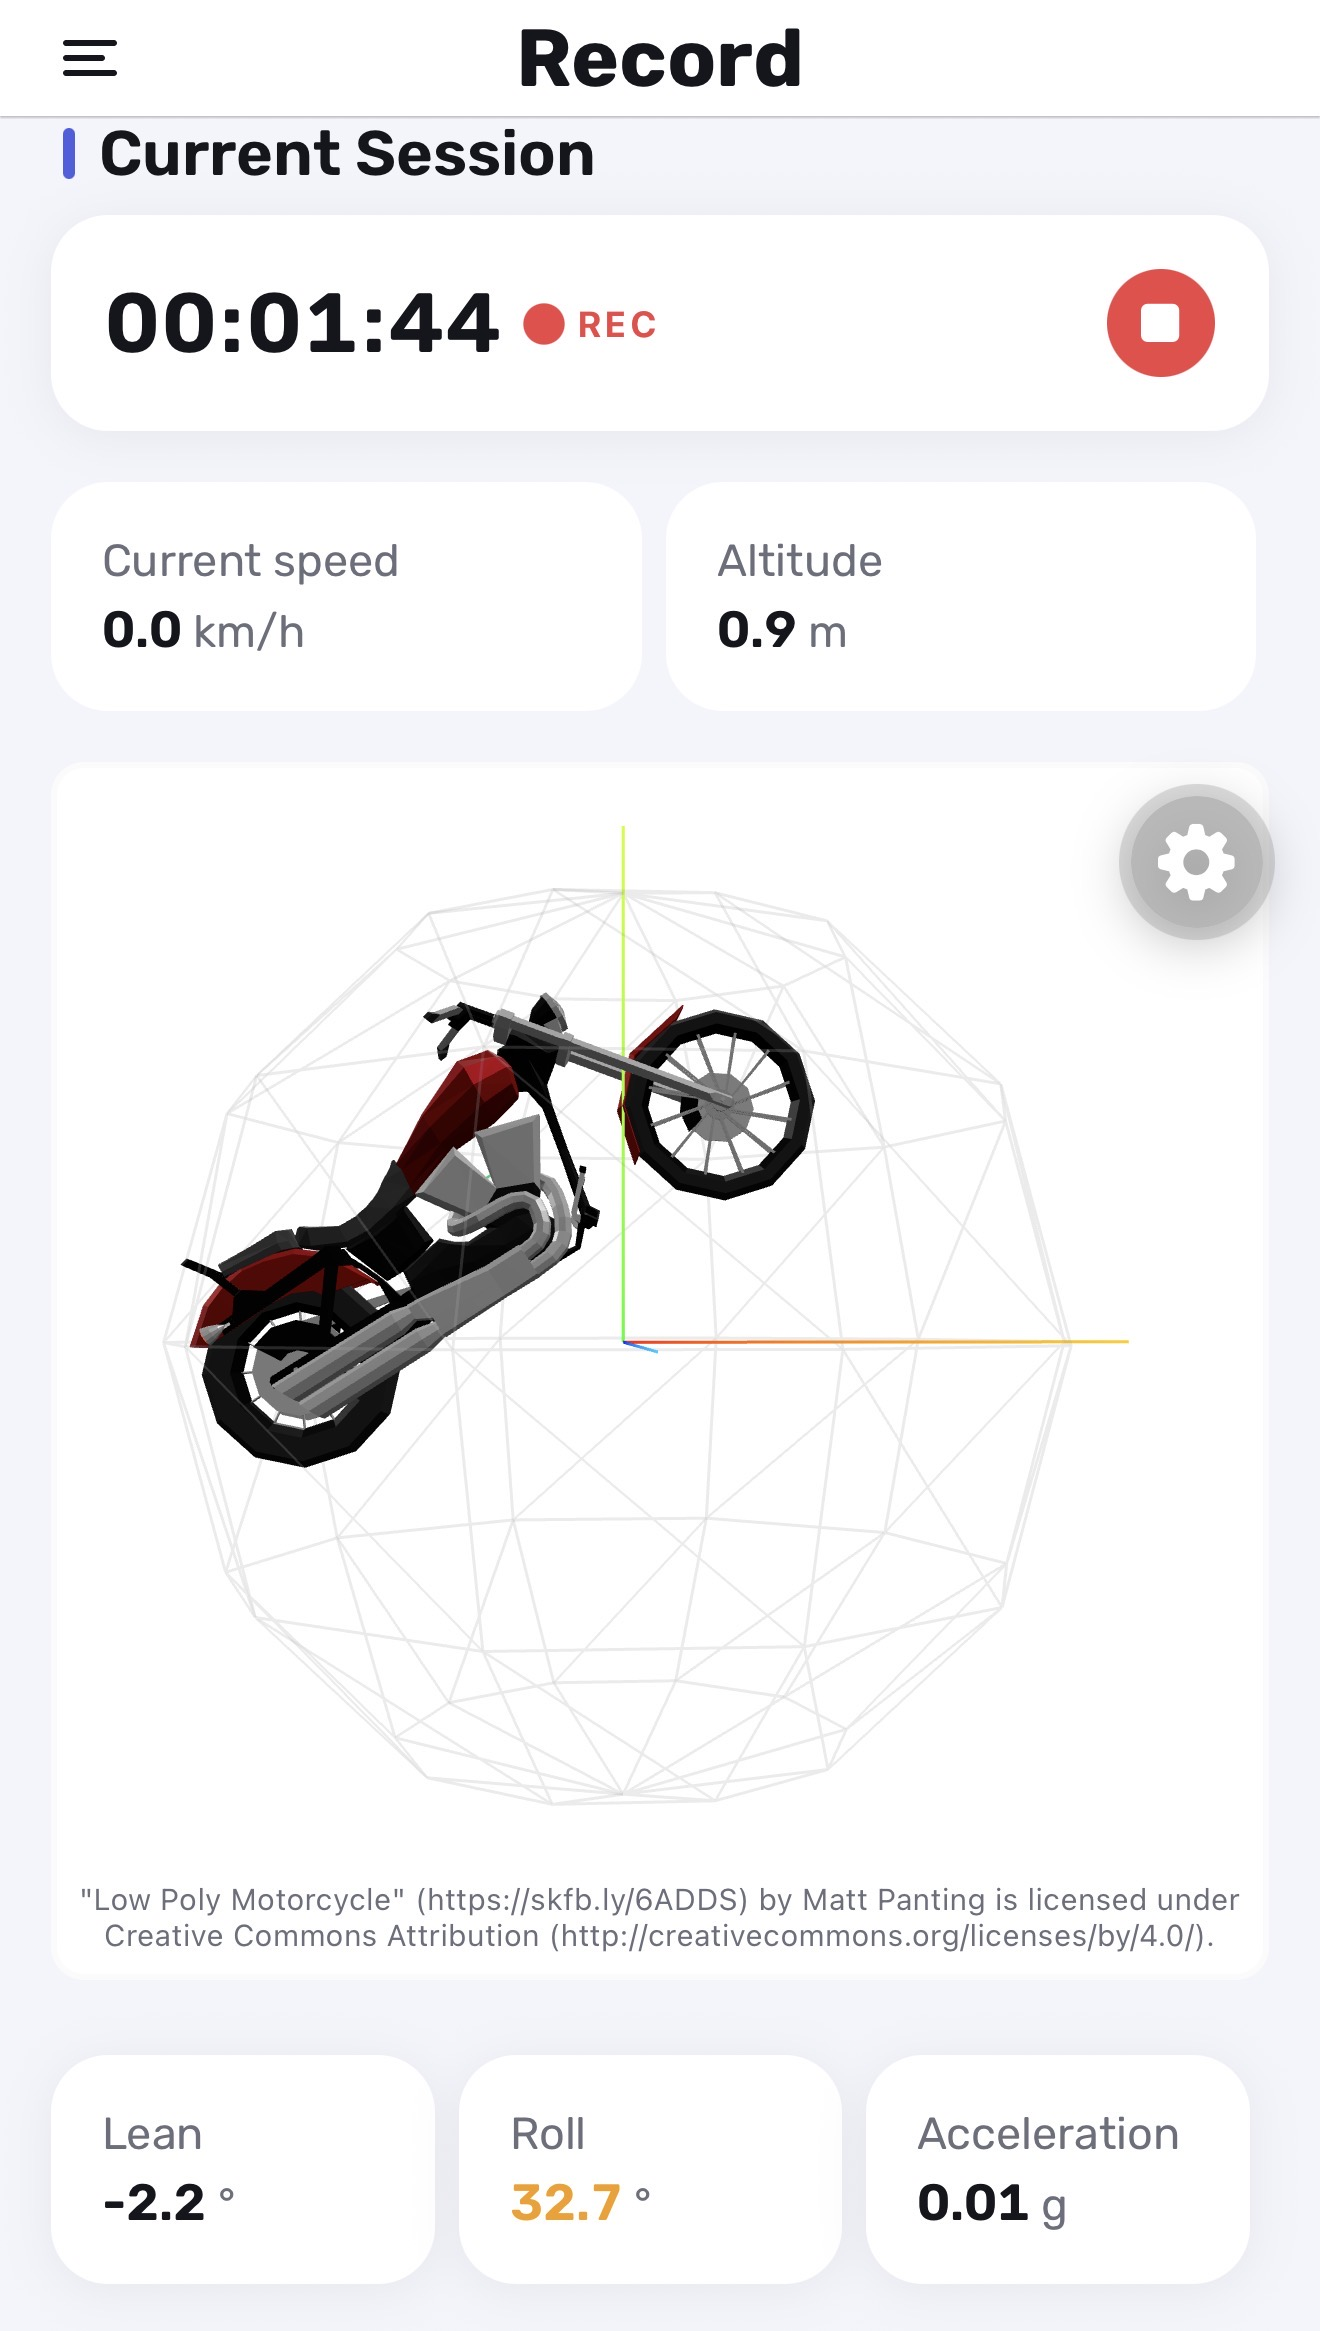
\includegraphics[width=0.4\textwidth]{../img/Applicazione/moto-3d.jpg}
    \caption{Visualizzazione 3D della moto, con assetto aggiornato in tempo reale}
\end{figure}

\newpage

\section{Segnalazione di microSD mancante durante la sessione}

\subsection{Richiamo alla scelta progettuale}

Questa sezione traduce in codice quanto descritto in
\hyperref[sec:app-sdmissing]{Segnalazione di microSD mancante durante la
sessione}: il componente presentazionale riutilizzato nei due contesti,
l'azione differenziata per contesto e il comportamento non richiudibile.

\subsection{Strutture dati e interfacce}

Il componente è parametrico rispetto a etichetta, colore e stato di
caricamento dell'azione proposta, senza contenere alcuna logica su quando
essere mostrato:

\begin{listing}[H]
\begin{minted}{tsx}
function SdMissingOverlay({
    onAction, actionLabel, actionLoading, actionColorStyle, loadingText
}: { ... }) { ... }
\end{minted}
\caption{Firma del componente presentazionale di segnalazione SD mancante}
\label{listing:sdmissing-props}
\end{listing}

\subsection{Dettagli implementativi}

\paragraph{Ripartizione dell'occupazione per sensore}
A differenza dei due overlay, che dipendono dal solo indicatore booleano di assenza scheda, questo componente legge dallo stesso oggetto di
dominio la percentuale di occupazione e l'indicatore di sovrascrittura di ciascun sensore, mostrandoli in una griglia:

\begin{listing}[H]
\begin{minted}{tsx}
{order.map(idx => {
    const percent = storageStatus.percentUsed[idx]
    const rewriting = storageStatus.rewriting[idx]
    return (
        <View key={idx}>
            <Text>{SENSOR_LABELS[idx]}</Text>
            <Text>{percent.toFixed(1)}%</Text>
            {rewriting && <Text>Rewriting</Text>}
        </View>
    )
})}
\end{minted}
\caption{Ripartizione per sensore della percentuale di occupazione}
\label{listing:storage-usage-card}
\end{listing}

L'ordine dei sensori nella griglia è fissato esplicitamente (\texttt{order}), invece di seguire l'ordine in cui i valori arrivano
dall'oggetto \texttt{StorageStatus}: una scelta che rende la disposizione stabile e prevedibile a schermo indipendentemente da come il
firmware serializza i dati sulla Characteristic. L'etichetta \texttt{Rewriting}, mostrata solo per i sensori configurati in modalità a
sovrascrittura che hanno già compiuto un giro completo del proprio buffer circolare, avvisa l'utente che, per quel sensore, i dati più vecchi
della sessione corrente sono già stati sostituiti da dati più recenti.

\begin{figure}[H]
    \centering
    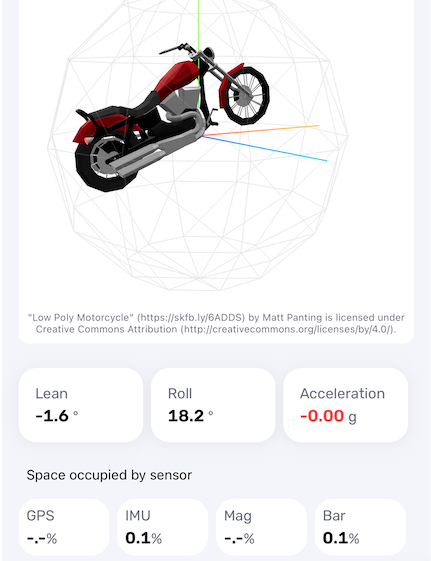
\includegraphics[width=0.4\textwidth]{../img/Applicazione/space_occupied.png}
    \caption{Ripartizione dell'occupazione per sensore, con indicatore di sovrascrittura}
\end{figure}

\paragraph{Stesso componente, azione differente per contesto}
Il componente compare in due punti della schermata Record, ciascuno con i
propri parametri: prima dell'avvio, offre un tentativo di ripetizione;
durante una sessione già in corso, offre solo l'arresto forzato:

\begin{listing}[H]
\begin{minted}{tsx}
// Prima dell'avvio: retry
{(startSdMissing || retrying) && (
    <SdMissingOverlay onAction={retryStartRecording} actionLabel="Retry"
        actionLoading={retrying} loadingText="Retrying..." ... />
)}

// Durante la sessione: arresto forzato
{storageStatus?.sdMissing && (
    <SdMissingOverlay onAction={() => stopRecording(activityName)}
        actionLabel="Block session" actionLoading={true} ... />
)}
\end{minted}
\caption{Le due invocazioni del componente, con azioni differenti}
\label{listing:sdmissing-usages}
\end{listing}

Nessun markup è duplicato tra i due casi: cambia solo quale funzione viene
passata come \texttt{onAction} e quale etichetta la accompagna, realizzando
lo Strategy Pattern descritto in progettazione senza introdurre due
componenti distinti.

\begin{figure}[H]
    \centering

    \begin{minipage}[t]{0.37\textwidth}
        \centering
        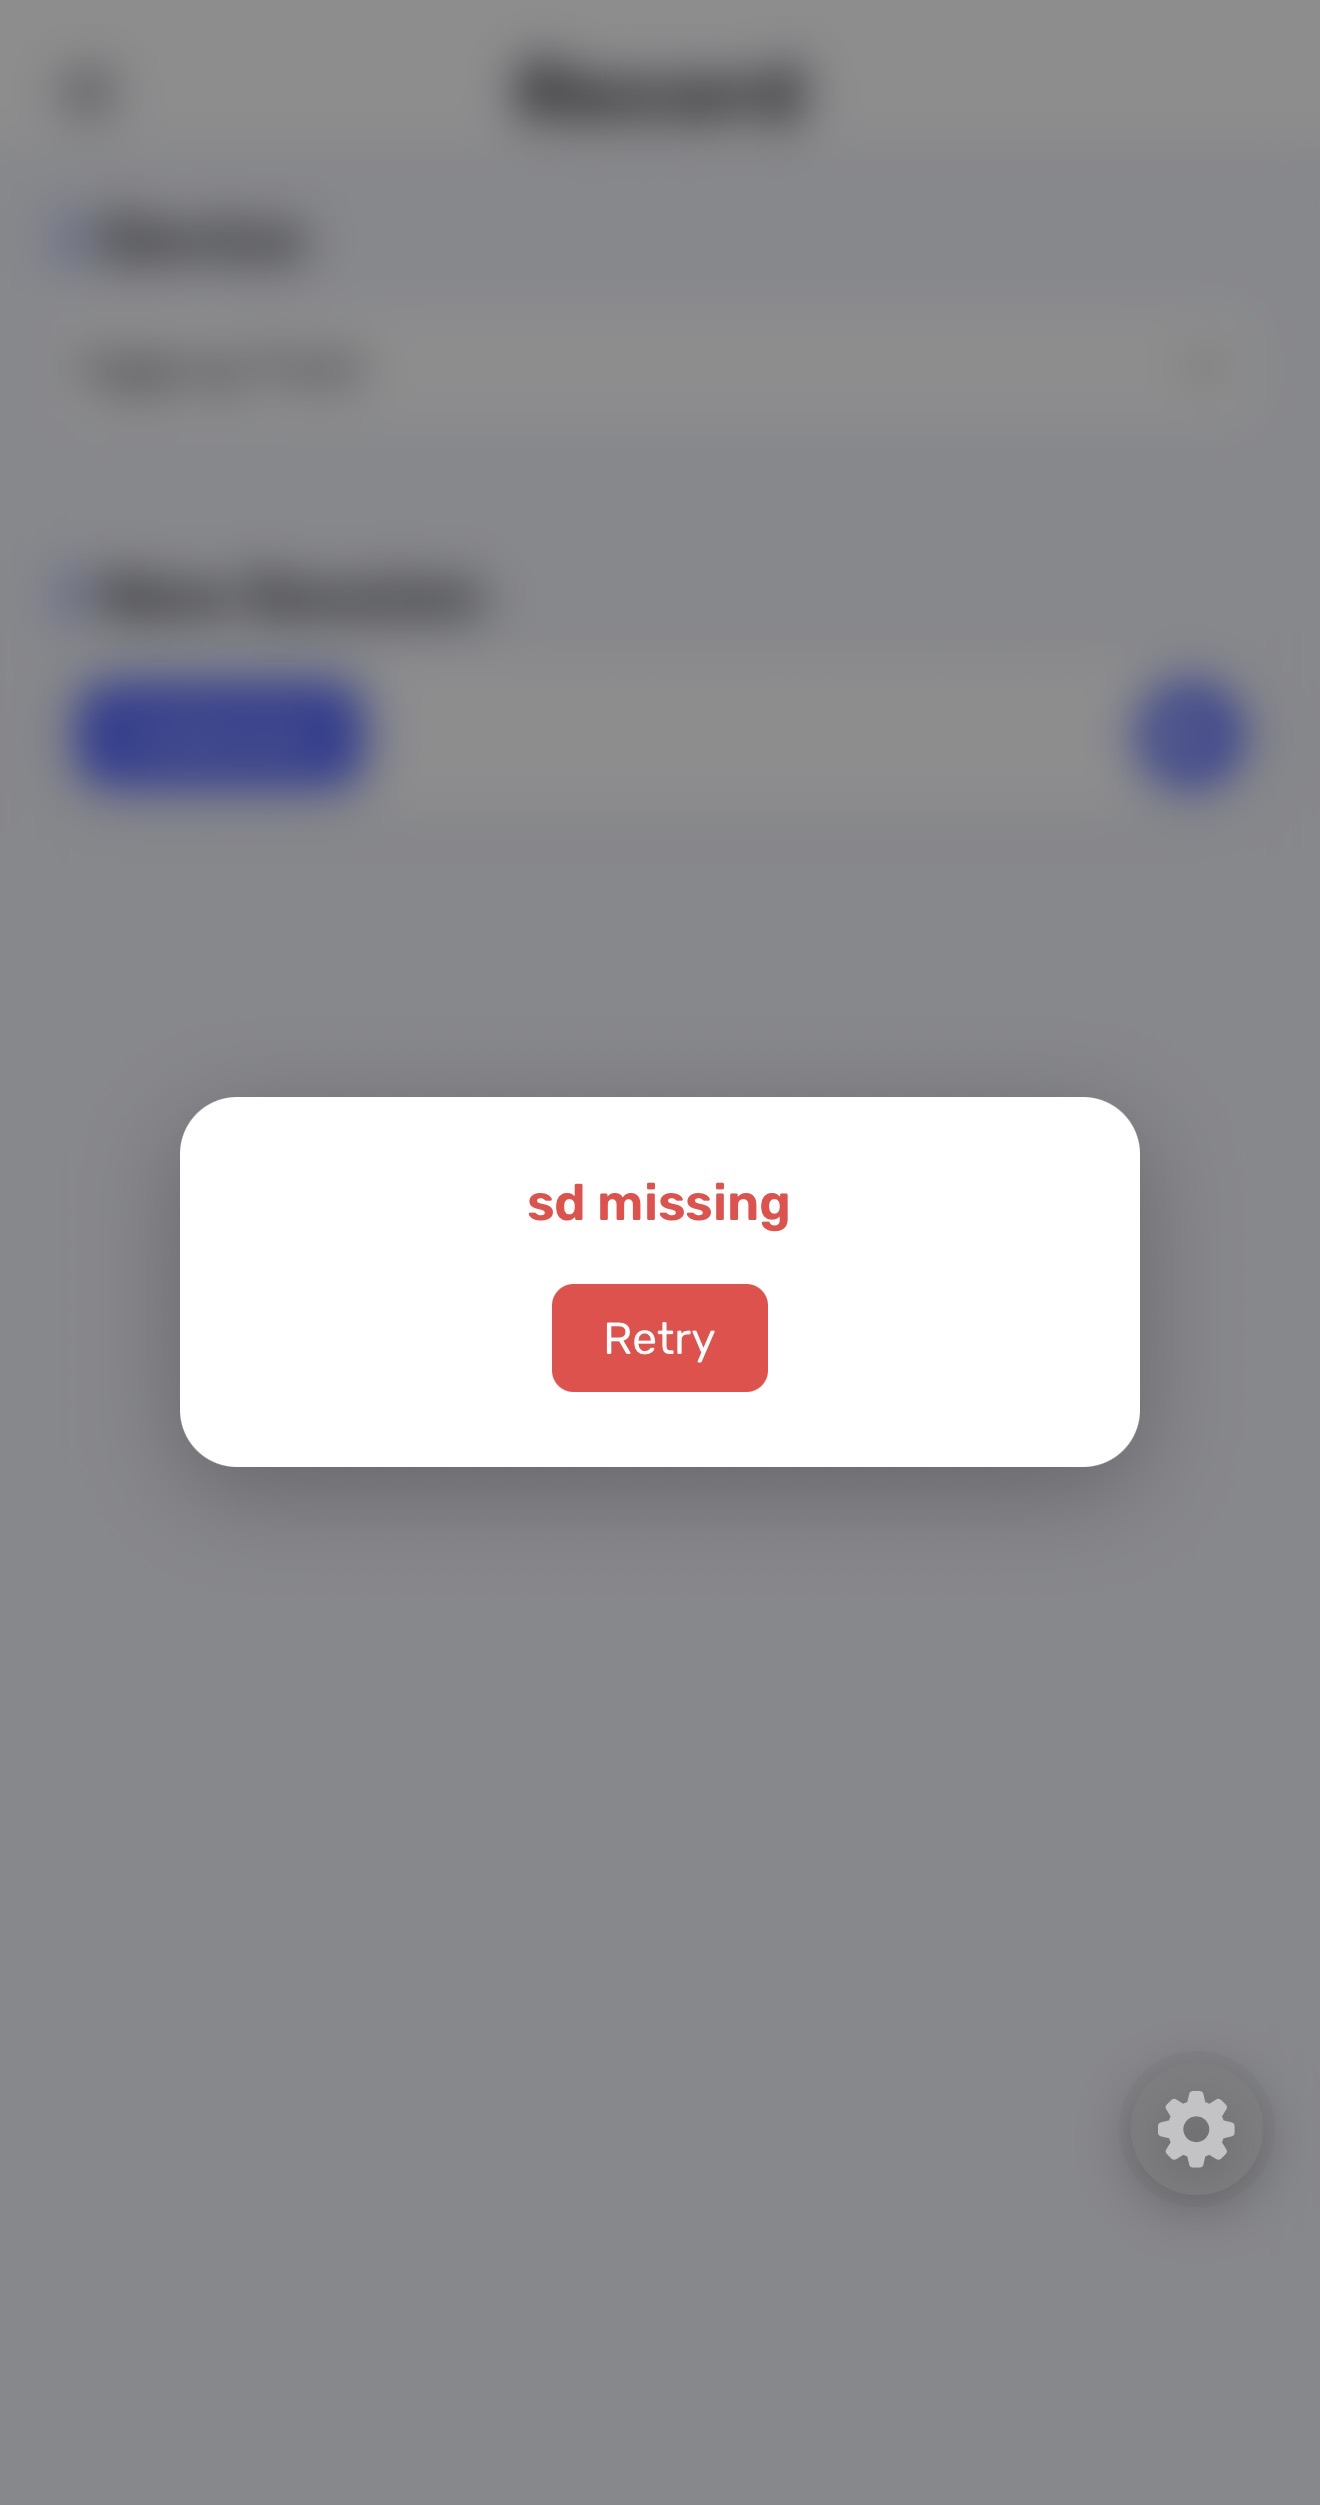
\includegraphics[width=\textwidth]{../img/Applicazione/sdmissing_preSession.jpg}

        \small (a) Retry prima dell'avvio
    \end{minipage}
    \hfill
    \begin{minipage}[t]{0.37\textwidth}
        \centering
        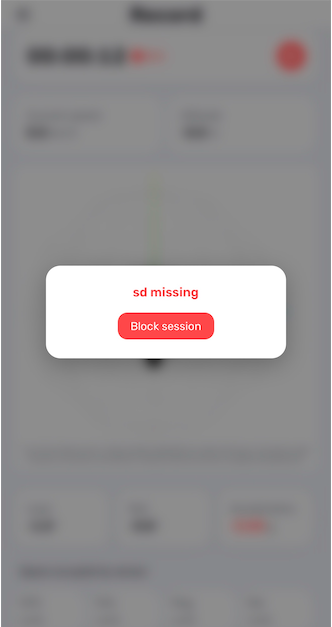
\includegraphics[width=\textwidth]{../img/Applicazione/sdmissing_midSession.png}

        \small (b) Arresto durante l'acquisizionee
    \end{minipage}

    \caption{I due utilizzi del componente \texttt{SdMissingOverlay}}
    \label{fig:sdmissing-usages}
\end{figure}

\paragraph{Impossibilità di chiusura senza azione}
Il componente è realizzato con un \texttt{Modal} a schermo intero, privo di
qualunque controllo di chiusura:

\begin{listing}[H]
\begin{minted}{tsx}
<Modal visible transparent animationType="fade">
    <View style={styles.sdOverlay}>
        <BlurView intensity={40} tint="dark" style={...} />
        <Text style={styles.sdOverlayTitle}>sd missing</Text>
        <Button title={actionLabel} onPress={onAction} showLoading={actionLoading} />
    </View>
</Modal>
\end{minted}
\caption{Overlay bloccante senza via di chiusura alternativa}
\label{listing:sdmissing-modal}
\end{listing}

L'unica interazione possibile con la schermata sottostante, finché la
condizione persiste, è quella offerta dal singolo pulsante del componente,
coerentemente con il Blocking Modal Pattern descritto in progettazione.

\paragraph{Scomparsa automatica al reinserimento della microSD}
Né il componente \texttt{SdMissingOverlay} né la schermata che lo ospita mantengono uno stato proprio su "SD mancante": la sua visibilità è
interamente derivata, a ogni render, dal valore corrente di \texttt{storageStatus.sdMissing}. Quando la scheda viene reinserita, è il firmware
stesso a rilevarlo ed eseguire il \hyperref[subsec:Recovery]{ripristino della sessione} già descritto lato firmware, ripubblicando poi lo stato di storage aggiornato.
Nell'app questo si traduce in un semplice cambio di valore della variabile booleana da cui dipende la condizione di rendering:

\begin{listing}[H]
\begin{minted}{tsx}
{storageStatus?.sdMissing && (
    <SdMissingOverlay onAction={() => stopRecording(activityName)}
        actionLabel="Block session" actionLoading={true} ... />
)}
\end{minted}
\caption{L'overlay scompare da solo non appena la condizione diventa falsa}
\label{listing:sdmissing-autoresume}
\end{listing}

\newpage

\section{Configurazione dei parametri del dispositivo}

\subsection{Richiamo alla scelta progettuale}

Questa sezione traduce in codice quanto descritto in
\hyperref[sec:app-config]{Configurazione dei parametri del dispositivo}:
l'Adapter/Facade Pattern che nasconde alla vista il significato di ogni
UUID e la codifica esplicita del valore scritto, applicati al selettore del
timeout di inattività dei sensori.

\subsection{Strutture dati e interfacce}

La vista non riceve mai un UUID grezzo da confrontare: riceve un oggetto di
dominio già pronto, e lo confronta solo con una costante nominata per
determinare se il parametro corrente è il timeout di inattività:

\begin{listing}[H]
\begin{minted}{tsx}
const isInactivityTimeout =
    item.getCharacteristicUUID() === BLE_CHARACTERISTICS.INACTIVITY_TIMEOUT
\end{minted}
\caption{Riconoscimento del parametro di timeout tramite l'oggetto di dominio}
\label{listing:config-selector}
\end{listing}

\subsection{Dettagli implementativi}

\paragraph{Un controllo dedicato per un insieme discreto di valori}
Il timeout di inattività non è un valore continuo su cui abbia senso uno
slider, ma un insieme chiuso di opzioni con etichetta (mai, 10, 30 o 60
minuti), coerentemente con quanto già descritto \hyperref[sec:inattivita]{lato firmware}: la vista
mostra quindi un menu a tendina:

\begin{listing}[H]
\begin{minted}{tsx}
const INACTIVITY_TIMEOUT_OPTIONS = [
    { label: 'Never', value: 0 },
    { label: '10 minutes', value: 10 },
    { label: '30 minutes', value: 30 },
    { label: '60 minutes', value: 60 },
]

{isInactivityTimeout && (
    <DropDownPicker items={INACTIVITY_TIMEOUT_OPTIONS} value={value}
        setValue={...} />
)}
\end{minted}
\caption{Menu a tendina per il timeout di inattività}
\label{listing:config-dropdown}
\end{listing}

L'etichetta mostrata accanto al valore riflette lo stesso caso speciale già
visibile nelle opzioni: il valore \texttt{0} non è mostrato come "0 minuti",
ma come \texttt{Never}, rendendo esplicito all'utente che quel valore
disabilita del tutto la sospensione dei sensori, non che ne azzera il tempo
di attesa.

\paragraph{Codifica esplicita immediatamente prima della scrittura}
Il valore numerico scelto dall'utente nel menu a tendina viene serializzato
secondo il formato concordato con il firmware solo nel punto in cui la
scrittura avviene effettivamente, non prima:

\begin{listing}[H]
\begin{minted}{tsx}
const toUint16Bytes = (v: number): number[] => {
    const buf = new ArrayBuffer(2)
    new DataView(buf).setUint16(0, v, true) // little-endian
    return Array.from(new Uint8Array(buf))
}
\end{minted}
\caption{Codifica del valore in un intero a 16 bit little-endian}
\label{listing:config-encode}
\end{listing}

Fino a questo punto il valore resta un semplice numero JavaScript, scelto
dall'utente tramite il menu a tendina senza alcuna conoscenza del formato di
trasmissione; è solo immediatamente prima della chiamata di scrittura sulla
Characteristic che il valore viene convertito nella rappresentazione a byte
attesa dal firmware, rendendo esplicito e localizzato in un solo punto il
contratto di formato tra le due parti.

\newpage